\documentclass[border=3pt]{standalone}
\usepackage[T1]{fontenc}
\usepackage{lmodern}
\usepackage{amsmath,amssymb}
\usepackage{tikz}
\usepackage{pgfplots}
\pgfplotsset{compat=1.17}
\usepgfplotslibrary{groupplots}
\usetikzlibrary{arrows.meta,calc,positioning,fit,backgrounds}

% Figure 1.1: tracking-by-detection pipeline with fixed operating points.
% Every processing block lists its input (In), its operation (Does) and its output (Out).
\newcommand{\blk}[4]{\textbf{#1}\\[-1pt]\rule{\linewidth}{0.4pt}\\[-2pt]
  \raggedright\textit{In:} #2\\ \textit{Does:} #3\\ \textit{Out:} #4}
\begin{document}
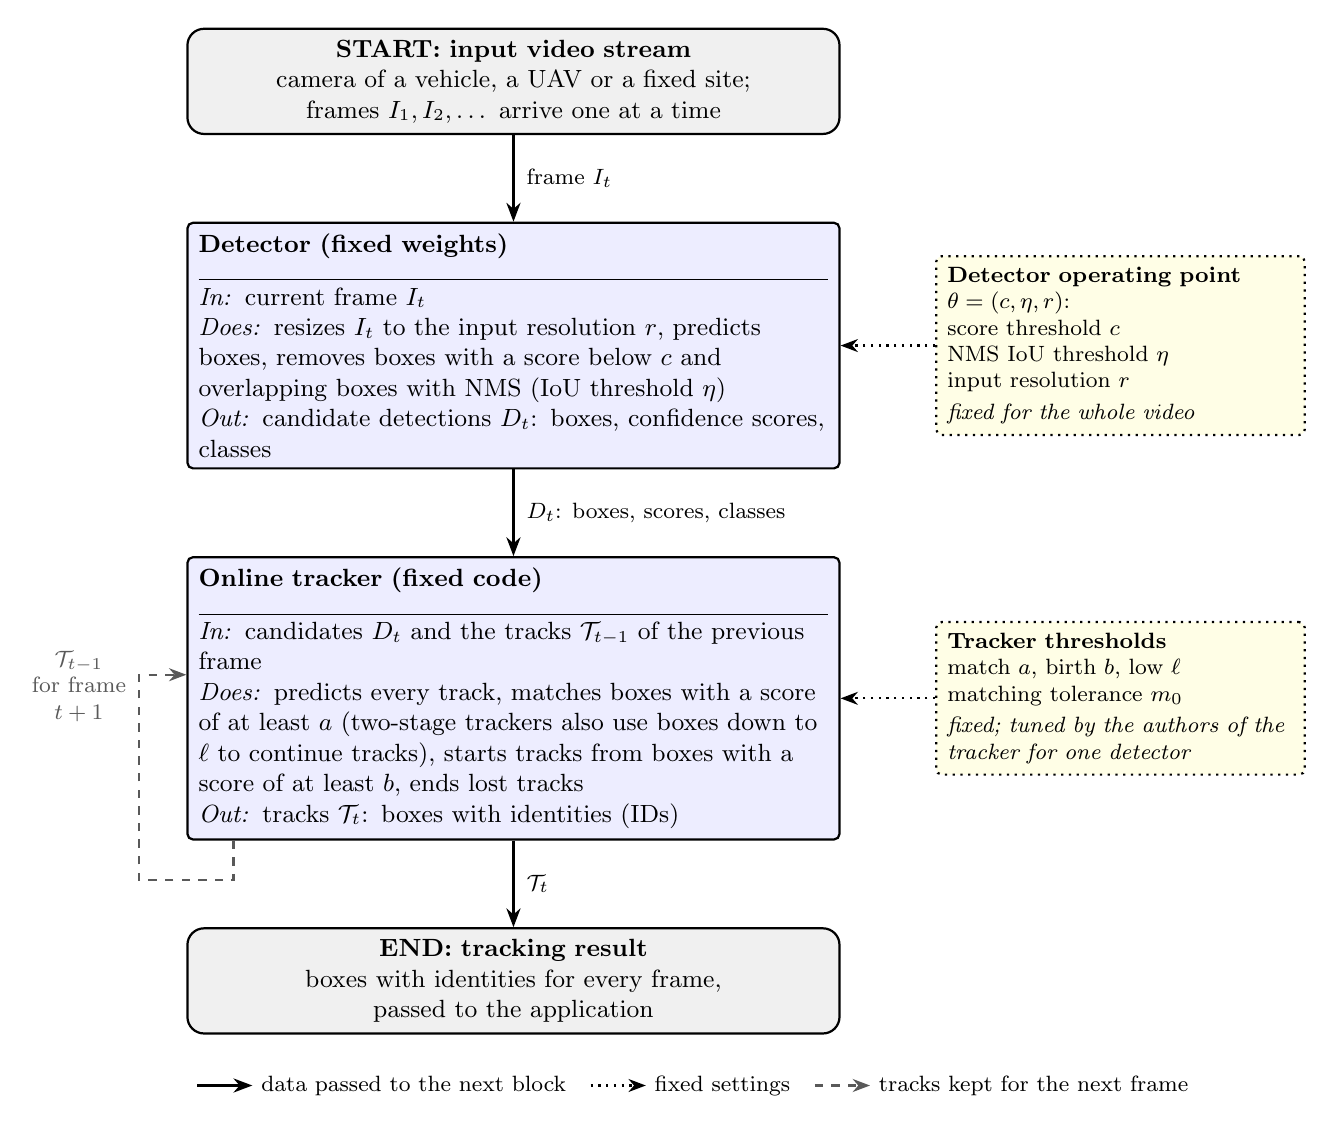
\begin{tikzpicture}[
  font=\small,
  io/.style={draw, thick, rounded corners=6pt, fill=gray!12, align=center, text width=80mm, inner sep=4pt},
  proc/.style={draw, thick, rounded corners=2pt, fill=blue!7, align=left, text width=80mm, inner sep=4pt},
  set/.style={draw, dotted, thick, rounded corners=2pt, fill=yellow!10, align=left, text width=44mm,
              font=\footnotesize, inner sep=4pt},
  arr/.style={-{Stealth[length=2.4mm]}, thick},
  ctl/.style={-{Stealth[length=2.2mm]}, thick, dotted},
  fb/.style={-{Stealth[length=2.2mm]}, thick, dashed, black!65},
  lab/.style={font=\footnotesize, fill=white, inner sep=1.5pt, align=center}]
% main path, top to bottom
\node[io] (in) {\textbf{START: input video stream}\\ camera of a vehicle, a UAV or a fixed site;\\
  frames $I_1, I_2, \dots$ arrive one at a time};
\node[proc, below=11mm of in] (det) {\blk{Detector (fixed weights)}
  {current frame $I_t$}
  {resizes $I_t$ to the input resolution $r$, predicts boxes, removes boxes with a score below $c$
   and overlapping boxes with NMS (IoU threshold $\eta$)}
  {candidate detections $D_t$: boxes, confidence scores, classes}};
\node[proc, below=11mm of det] (trk) {\blk{Online tracker (fixed code)}
  {candidates $D_t$ and the tracks $\mathcal{T}_{t-1}$ of the previous frame}
  {predicts every track, matches boxes with a score of at least $a$ (two-stage trackers also use
   boxes down to $\ell$ to continue tracks), starts tracks from boxes with a score of at least $b$,
   ends lost tracks}
  {tracks $\mathcal{T}_t$: boxes with identities (IDs)}};
\node[io, below=11mm of trk] (out) {\textbf{END: tracking result}\\ boxes with identities for every frame,\\
  passed to the application};
% fixed settings on the right
\node[set, right=12mm of det] (dset) {\textbf{Detector operating point}\\ $\theta=(c,\eta,r)$:\\
  score threshold $c$\\ NMS IoU threshold $\eta$\\ input resolution $r$\\[2pt] \textit{fixed for the whole video}};
\node[set, right=12mm of trk] (tset) {\textbf{Tracker thresholds}\\ match $a$, birth $b$, low $\ell$\\
  matching tolerance $m_0$\\[2pt] \textit{fixed; tuned by the authors of the tracker for one detector}};
% arrows
\draw[arr] (in) -- node[lab, right=1mm] {frame $I_t$} (det);
\draw[arr] (det) -- node[lab, right=1mm] {$D_t$: boxes, scores, classes} (trk);
\draw[arr] (trk) -- node[lab, right=1mm] {$\mathcal{T}_t$} (out);
\draw[ctl] (dset.west) -- (det.east |- dset.west);
\draw[ctl] (tset.west) -- (trk.east |- tset.west);
\draw[fb] ($(trk.south west)+(6mm,0)$) -- ++(0,-5mm) -| ([xshift=-6mm]trk.west)
  |- node[lab, pos=0.25, left=1mm] {$\mathcal{T}_{t-1}$\\for frame\\$t+1$} ([yshift=3mm]trk.west);
% legend
\node[font=\footnotesize, align=left, anchor=north west] at ($(out.south west)+(0,-4mm)$) {%
  \tikz[baseline=-0.6ex]\draw[arr] (0,0) -- (7mm,0); data passed to the next block\quad
  \tikz[baseline=-0.6ex]\draw[ctl] (0,0) -- (7mm,0); fixed settings\quad
  \tikz[baseline=-0.6ex]\draw[fb] (0,0) -- (7mm,0); tracks kept for the next frame};
\end{tikzpicture}
\end{document}
